\chapter[Problem-Solving Strategies]{Problem-Solving Strategies for SAT Math Sections}

\subsection{Worksheet 1D: Warm-Up Problems}

\bigskip
\textbf{\underline{Algebra and Data Analysis Vocabulary}: Read the words and definitions (if you don't already know them) and then answer the question that follows.}

\begin{enumerate}[label=\bfseries\arabic*.]
\item \textbf{Constant} - A value represented by a variable that will not change

\bigskip
The constant $a$ represents the speed in miles per hour that a car can drive. If said car drives 125 miles in 2.5 hours, what is the value of $a$?

\vfill
\item \textbf{Expression} - A function or any combination of constants. Solve the expression when $x$ is equal to six: $3x+7$

\vfill
\item \textbf{Distributed equally} - Split up in equal parts and given to multiple people

\bigskip
A rectangular pizza measuring 80 cm long and 60 cm wide is cut into square pieces each with an area of 400 cm$^2$ and distributed equally among 4 friends. How many pieces did each person get?

\vfill
\item \textbf{Set of integers, elements} - A set is a group of numbers. The numbers within the set are referred to as elements.

\bigskip
How many elements in the set of the first 8 prime numbers have 3 in their one's digit?

\vfill
\item \textbf{Domain, Range} - The domain is the set of all possible $x$ values. The range represents all possible $y$ values.

\bigskip
What is the domain and range of the following equation $y=|3x+5|$

\vfill
\item \textbf{Average/Arithmetic mean, median, mode} - In a set of numbers the average is the sum of all values divided by the number of values. The median is the middle value. The mode is the most common value.

\bigskip
Find the mean, median, and mode of this set of numbers:

\[10,20,20,40,50,90,120\]

Mean:

\medskip
Median:

\medskip
Mode:
\end{enumerate}

\vfill
\pagebreak
\section[SAT Algebra]{General Strategies for SAT Algebra}

It can be difficult to know every concept on the SATs or more frequently, which topic(s) is best used to solve the problem. Therefore, if you get to a problem that you don't know how to solve, then you can use the following strategies to help you find the right answer. They spell the acronym PUFS (like the tissue company but with only 1 letter ``F'').

\bigskip
\textbf{\large P}lug in real numbers

\medskip
\textbf{\large U}se the answer choices

\medskip
\textbf{\large F}ormulas

\medskip
\textbf{\large S}ee the problem

\hrulefill

\textbf{SAT Math Strategy 1: Plug in real number}

\bigskip
Many SAT problems are made unnecessarily tricky by using \longline instead of \longline.

\begin{enumerate}
\item Assigning each variable a unique, \longline (for example, if there are variables $a, b$, and $c$ in the problem, make $a=2, b=3, c=5$). These numbers should be easy to work with. If you are using percentages, it is recommended to use \longline for the base variable because percentages are out of 100.
\item Solve the problem with these \longline instead of variables.
\item If necessary, translate the numbers back to \longline, percentages, fractions, etc
\end{enumerate}

\textbf{Try It:} If $a$ is 1/3 of $b$ and $b$ is 2/5 of $z$ and $z>0$, then $a$ is what percentage of $z$?

\pagebreak
\subsection{SAT Worksheet 2D: 6 Questions, 8 Minutes}

\begin{multienumerate}
\mitemxx{\basic

Which of the following could be the remainders when 3 consecutive, even, positive integers are each divided by 5?

\begin{enumerate}[label=(\Alph*)]
\item $1,2,3$
\item $1,4,6$
\item $0,1,4$
\item $1,3,0$
\item $2,3,4$
\end{enumerate}}{\basic

If $(1/5)a+b=b^2-a$, what is $a$ in terms of $b$?

\begin{enumerate}[label=(\Alph*)]
\item $b^2-b$
\item $5(b^2-b)$
\item $1/5(b^2-b)$
\item $b-\sqrt{b}$
\item $5/6(b^2-b)$
\end{enumerate}}

\vfill
\mitemxx{\medium

When some integer $b$ is divided by 4, the remainder is 3. How many values of $b$ are between 0 and 40?

\begin{enumerate}[label=(\Alph*)]
\item Five
\item Seven
\item Eight
\item Nine
\item Ten
\end{enumerate}}{\medium

\medskip
\begin{tabular}{|l|c|c|c|}\hline
& Bus & Non-bus & \textbf{Total}\\\hline
9\textsubscript{th} graders & A & B & C\\\hline
10\textsubscript{th} graders & D & E & F\\\hline
11\textsubscript{th} graders & G & H & I\\\hline
\textbf{Total} & J & K & L\\\hline
\end{tabular}

\medskip
The chart above has a letter to represent the number of students in each category. Which of the following equals $A$?

\begin{enumerate}[label=(\Alph*)]
\item $I-(G+E)-B$
\item $F-E+D$
\item $J-(I-H)-D$
\item $H-E-(C-B)$
\item None of the above
\end{enumerate}}

\vfill
\mitemxx{\advanced

If $a$ and $b$ are positive integers and $4^a=2^b/2$, what is $a$ in terms of $b$?

\begin{enumerate}[label=(\Alph*)]
\item $b/2$
\item $b^{1/2}$
\item $b$
\item $(b-1)/2$
\item $2b$
\end{enumerate}}{\advanced

The ratio of fruit juice to water in Betty's orange juice is $7:3$. How many liters of fruit juice is in 2 liters of Betty's orange juice?}
\end{multienumerate}

\pagebreak
\textbf{SAT Math Strategy 2: Use the answer choices}

If the question is multiple choice, then you may be able to plug in the answer choices into the question to see which answer choice gives you the correct answer.

\bigskip
Hint: It is suggested in SAT literature that if you try this approach, that you should start with answer choice C and work outwards or answer choice E and go backwards from E to A because the SATs will rarely make problems that can be solved with this strategy to have answer choice A. 

\bigskip
\textbf{Try It:} What is the smallest of 5 consecutive even integers if the sum of these integers equals 300?

\begin{enumerate}[label=(\Alph*)]
\item 50
\item 52
\item 54
\item 56
\item 58
\end{enumerate}

\newpage
\subsection{SAT Worksheet 3D: 4 Problems, 5 Minutes}

\begin{multienumerate}
\mitemxx{\medium

If $a$ is a positive integer, what is the smallest value of $a$ for which $a^2+1.5a$ is an integer?

\begin{enumerate}[label=(\Alph*)]
\item 1/3
\item 1/2
\item 1
\item 2
\item 3
\end{enumerate}}{\medium

A salesman receives \$500 per week and a 5\% commission on each car he sells. If he sold 18 cars at the same price and earned \$3600 in one month, what is the price of 1 car that he sold? (1 month = 4 weeks)

\begin{enumerate}[label=(\Alph*)]
\item \$1,777.78
\item \$3,444.44
\item \$4,000.00
\item \$32,000.00
\item Cannot be determined from the information given
\end{enumerate}}

\vfill
\mitemxx{\advanced

Function $f$ is defined as $f(t)=t-4$ and function $g$ is defined as $g(t)=t^2-32$. For what value of $t$ does $2f(t)=g(t)$?

\begin{enumerate}[label=(\Alph*)]
\item $-6$
\item $-4$
\item 0
\item 2
\item 4
\end{enumerate}}{\advanced

You are given that $(x+2)(x-b)=x^2+cx-8$ where $b$ and $c$ are constants. What is the value of $1/2c$

\begin{enumerate}[label=(\Alph*)]
\item $-2$
\item $-1$
\item 1
\item 2
\item 8
\end{enumerate}}
\end{multienumerate}

\vfill
\pagebreak
\textbf{SAT Math Strategy \#3: Quickly recall and write down general formulas}

Look at the formulas that are given on the SATs and memorize the ones that aren't. Fill in the formulas below that are not given on the SAT test:

\bigskip
Formula for directly proportional:

\bigskip
Formula for inversely proportional:

\bigskip
Formula for average:

\bigskip
Formula for slope:

\bigskip
Formula for equation of a line:

\bigskip
**When you get to a problem that calls for a topic with a formula associated with it, write the general formula in words on your test booklet. For example, if there was a question that has to do with averages we would write down \longline. Then, rewrite the formula with the numbers or variables from the problems filled in.**

\vfill
\textbf{Try it:} 30\% of the students in Ms. Law's class had an average test score of 78 points. The rest of the class had an average test score of 84 points. What is the average test score for all students in Ms. Law's class?

\begin{enumerate}[label=(\Alph*)]
\item 79.5
\item 81.0
\item 82.2
\item 83.0
\item 83.1
\end{enumerate}

\vfill
\newpage
\subsection{SAT Worksheet 4D: 4 Questions, 5 Minutes}

\begin{multienumerate}
\mitemxx{\basic

If $y$ is directly proportional to $x$ and $y=-7$ when $x=2$, what is the value of $x$ rounded to the closest integer when $y=2$?

\begin{enumerate}[label=(\Alph*)]
\item $-7$
\item $-2$
\item $-1$
\item 0
\item 2
\end{enumerate}}{\basic

If $y$ is inversely proportional to $x$ and $y=-7$ when $x=2$, what is the value of $x$ when $y=5.5$?

\begin{enumerate}[label=(\Alph*)]
\item $-2.55$
\item $-1.57$
\item $-0.61$
\item $-0.27$
\item 1
\end{enumerate}}

\vfill
\mitemxx{\medium

If the average of $2a$ and $1/3a$ is 6, what is the value of $5a$?}{\medium

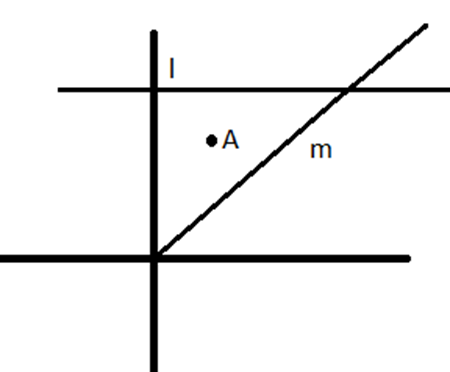
\includegraphics{48}


In the figure above, line $m$ has a slope of 3/4 and the equation of line $l$ is $y=5$. If A is between line $m$ and line $l$ and the $x$-coordinate of point $A$ is 2, how many possible integer values are there for the $y$-coordinate of point $A$?

\begin{enumerate}[label=(\Alph*)]
\item 0
\item 1
\item 2
\item 3
\item More than 3
\end{enumerate}}
\end{multienumerate}

\newpage
\textbf{SAT Math Strategy 4: See and solve the problem using visuals like diagrams, charts, or tables}

\bigskip
Drawing a diagram, table, or chart can help you to visualize the problem, particularly for

\longline and \longline problems. They don't need to be detailed or drawn perfectly-just enough to for you to see the information that you currently have and what you need to solve for.

\bigskip
\textbf{Try It:} 5 students are going to be lined up against a wall. In how many different ways can the 5 students be arranged in a row?

\begin{enumerate}[label=(\Alph*)]
\item 5
\item 24
\item 25
\item 100
\item 120
\end{enumerate}

\newpage
\subsection{SAT Worksheet 5D: 6 Questions, 8 Minutes}

\begin{multienumerate}
\mitemxx{\basic

The ratio of the interior angles in a quadrilateral is $2:5:6:10$. What is the positive difference between the smallest and the largest angle?}{\basic

For example, 3 tennis balls numbered 1-3 and 4 tennis rackets are numbered 1-4, how many different combinations of 1 tennis ball and 1 tennis rackets are possible?

\begin{enumerate}[label=(\Alph*)]
\item 6
\item 7
\item 12
\item 16
\item 24
\end{enumerate}}

\vfill
\mitemxx{\medium

At Jamestown high school, there are 500 students.  20\% of students study biology and 50\% more students study psychology than biology. If 40 students study both biology and psychology, what is the number of Jamestown high school students that do not study biology or psychology?}{\medium

The points $RST$ are colinear and appear in that order. $RT=28$ and $RS=1/3ST$. Point $U$ is then drawn so that it is the midpoint of $RS$ and point $V$ is drawn between  $S$ and $T$ so that $SV=4/5ST$. What is the length of $UV$?   %I clarified the location of SV here

\begin{enumerate}[label=(\Alph*)]
\item 10.5
\item 14.2
\item 17.2
\item 20.3
\item 21
\end{enumerate}}

\vfill
\mitemxx{\advanced

The area of an equilateral triangle $ABC$ is twice the size of the perimeter of equilateral triangle $DEF$. If one side length of $DEF$ is 6 2/3 inches, what is the length of one side in the triangle $ABC$, in inches, rounded to the nearest hundredth?}{\advanced

Abby, Biana, Colin, David, and Ed are going to be lined up against a wall. In how many different ways can the 5 students be arranged in a row if Ed can not be first or last in line?

\begin{enumerate}[label=(\Alph*)]
\item 10
\item 25
\item 72
\item 96
\item 120
\end{enumerate}}
\end{multienumerate}

\newpage
\subsection{SAT Worksheet 6D (Basic): 6 Questions, 8 Minutes}

\begin{multienumerate}
\mitemxx{Which of the following numbers when square rooted, is greater than itself?

\begin{enumerate}[label=(\Alph*)]
\item 1/2
\item 3/4
\item 4/3
\item 5/4
\item 6/5
\end{enumerate}}{If $3x+ky=1$ has a slope of $-2$, what is the value of $k$?

\begin{enumerate}[label=(\Alph*)]
\item $-6$
\item $-3/2$
\item 2/3
\item 3/2
\item 6
\end{enumerate}}

\vfill
\mitemxx{If $k$ is an even integer, which of the following must also be even?

\begin{enumerate}[label=(\Alph*)]
\item $k/2$
\item $2k+1$
\item $k^2$
\item $k^3-3$
\item $k+1/3$
\end{enumerate}}{If $f(2)=10$ and $f(4)=6$, which of the following is a linear model of $f(n)$?

\begin{enumerate}[label=(\Alph*)]
\item $-2n+14$
\item $2n+6$
\item $-1/2n+11$
\item $1/2n+9$
\item $2/3n+1/3$
\end{enumerate}}

\vfill
\mitemxx{If $x<0$ and $y\neq0$, which of the following expressions must be a positive number?

\begin{enumerate}[label=(\Alph*)]
\item $x/y$
\item $xy$
\item $y-x$
\item $x^2y$
\item $(x+y)^2$
\end{enumerate}}{A coat is on sale for 20\% off of the original price after a month. After another month, the price falls an additional 10\% off of the sale price. What percent of the original price is the sale price?

\begin{enumerate}[label=(\Alph*)]
\item 72\%
\item 78\%
\item 80\%
\item 82\%
\item 88\%
\end{enumerate}}
\end{multienumerate}

\newpage
\subsection{SAT Worksheet 7D (Medium): 6 Questions, 9 Minutes}

\begin{multienumerate}
\mitemxx{If $\frac{3}{k+2}-\frac{1}{k}=\frac{1}{5k}$, what is the value of $k$?

\begin{enumerate}[label=(\Alph*)]
\item 3/4
\item 1
\item 4/3
\item 2
\item 5/2
\end{enumerate}}{If $10^{n-3}=100^{m+1}$, what is the value of $n-2m$?

\begin{enumerate}[label=(\Alph*)]
\item 2
\item 2.5
\item 4
\item 4.5
\item 5
\end{enumerate}}

\vfill
\mitemxx{3.	Points $ABCD$ are collinear such that $B$ is halfway between $A$ and $C$ and $C$ is halfway between $B$ and $D$. If the total distance between $A$ and $D$ is 12, what is the distance between $B$ and $D$?

\begin{enumerate}[label=(\Alph*)]
\item 3
\item 4
\item 6
\item 8
\item 9
\end{enumerate}}{A cell phone tower sits on a corner of a square of length $n$ miles. If three sub towers lie on the other corners of the square, which expression indicates the sum of the distances of the sub towers from the main tower?

\begin{enumerate}[label=(\Alph*)]
\item $2n+\sqrt{2}n$
\item $n^2$
\item $3n$
\item $3n+\sqrt{2}n$
\item $4n$
\end{enumerate}}

\vfill
\mitemxx{Quadrilateral $ABCD$ has $\angle A = \angle B = \angle C = 1/2\angle D$, and $\angle D = 1/2\angle A$. What is the value of $\angle D$?

\begin{enumerate}[label=(\Alph*)]
\item $45^\circ$
\item $48^\circ$
\item $72^\circ$
\item $90^\circ$
\item $144^\circ$
\end{enumerate}}{

\medskip
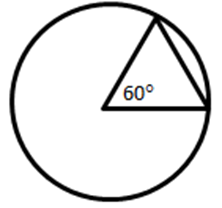
\includegraphics{49}

In the diagram above, the perimeter of the triangle is 9. What is the circumference of the circle?

\begin{enumerate}[label=(\Alph*)]
\item $3\pi$
\item 6
\item $6\pi$
\item 9
\item $9\pi$
\end{enumerate}}
\end{multienumerate}

\newpage
\subsection{SAT Worksheet 9D (Advanced): 6 Questions, 10 Minutes}
\begin{multienumerate}
\mitemxx{The diagonals of a rectangle are equal to twice the length of the shortest side. If $w$ is the shortest side and $l$ is the longer side, which expression represents the value of $l$ in terms of $w$?

\begin{enumerate}[label=(\Alph*)]
\item $\sqrt{2}w$
\item $\sqrt{2}w/2$
\item $\sqrt{3}w$
\item $\sqrt{3}w/3$
\item $\sqrt{5}$
\end{enumerate}}{If the system

\[6x-4y=15\]

\[3x+k^2y=12\]

Represents the equations of perpendicular lines, what must be the value of $k$?

\begin{enumerate}[label=(\Alph*)]
\item $\pm2/3$
\item $\pm 3/2$
\item $\pm\sqrt{2}/2$
\item $\pm2\sqrt{3}/3$
\item $\pm3\sqrt{2}/2$
\end{enumerate}}

\vfill
\mitemxx{The average of 10 numbers is 16. If the average of 6 of the numbers is 8, what is the average of the remaining numbers?

\begin{enumerate}[label=(\Alph*)]
\item 24
\item 26
\item 28
\item 29.5
\item 56
\end{enumerate}}{If $x$ is a positive integer, and

\[\sqrt{x}+\sqrt{2x+1}=x+1\]

What is the value of $2x$?

\begin{enumerate}[label=(\Alph*)]
\item 0
\item 2
\item 4
\item 6
\item 8
\end{enumerate}}

\vfill
\mitemxx{If the greatest common factor of $m$ and $n$ is $q$, then $q$ is also the greatest common factor of $m$ and which expression?

\begin{enumerate}[label=(\Alph*)]
\item $n-1$
\item $2n$
\item $n^2$
\item $n+1$
\item $m-n$
\end{enumerate}}{There is a total of \$2.20 in quarters, nickels, and dimes. If there are twice as many nickels and twice as many dimes as there are quarters, what is the total value of the dimes?

\begin{enumerate}[label=(\Alph*)]
\item \$0.20
\item \$0.40
\item \$0.60
\item \$0.80
\item \$0.90
\end{enumerate}}
\end{multienumerate}